%\documentclass[12pt,preprint]{aastex}
\documentclass[iop,apj]{emulateapj}
%\usepackage{multirow}
\usepackage{longtable}
\usepackage{ulem}
%\usepackage[monochrome]{color}
\usepackage{color}
%\usepackage{lipsum}
\usepackage{amsmath}
%\usepackage{hyperref}

\newcommand{\eqqref}[1]{Equation (\ref{#1})}
\newcommand{\tabref}[1]{Table~\ref{#1}}
\newcommand{\figref}[1]{Figure~\ref{#1}}
\newcommand{\secref}[1]{Section~\ref{#1}}
\newcommand{\appref}[1]{Appendix~\ref{#1}}

\newcommand{\SNeIa}{SNe~Ia}
\newcommand{\SNIa}{SN~Ia}
\newcommand{\C}[1]{\ensuremath{{}^{#1}{\rm C}}}
\newcommand{\Ox}[1]{\ensuremath{{}^{#1}{\rm O}}}
\newcommand{\Ne}[1]{\ensuremath{{}^{#1}{\rm Ne}}}
\newcommand{\Na}[1]{\ensuremath{{}^{#1}{\rm Na}}}
\newcommand{\Mg}[1]{\ensuremath{{}^{#1}{\rm Mg}}}
\newcommand{\Ni}[1]{\ensuremath{{}^{#1}{\rm Ni}}}
\newcommand{\Co}[1]{\ensuremath{{}^{#1}{\rm Co}}}
\newcommand{\Si}[1]{\ensuremath{{}^{#1}{\rm Si}}}
\newcommand{\Fe}[1]{\ensuremath{{}^{#1}{\rm Fe}}}
\newcommand{\code}[1]{\textsc{#1}}
\newcommand{\FLASH}{\code{FLASH}}
\newcommand{\CASTRO}{\code{CASTRO}}
\newcommand{\MESA}{\code{MESA}}
\newcommand{\PARAMESH}{\code{PARAMESH}}
\newcommand{\pv}{\ensuremath{\phi}}
\newcommand{\bvec}[1]{\ensuremath{\boldsymbol{#1}}} %boldface vector style
\newcommand{\grad}{\bvec{\nabla}} %gradient
\newcommand{\curl}{\bvec{\nabla \times}} %curl
\newcommand{\Atwood}{\ensuremath{\mathrm{At}}}
\newcommand{\adndt}{At.~Data~Nucl.~Data~Tables}
\newcommand{\At}{{\rm At}}
\newcommand{\ee}[1]{\ensuremath{\times 10^{#1}}}
\newcommand{\cdens}{\rho_{c}}

% basic unit typesetteing
\newcommand{\unitspace}{\ensuremath{\,}}
\newcommand{\usp}{\unitspace}
\newcommand{\numberspace}{\ensuremath{\;}}
\newcommand{\nsp}{\numberspace}
\newcommand{\unitstyle}[1]{\ensuremath{\mathrm{#1}}}
\newcommand{\power}[2]{\ensuremath{{#1}^{#2}}}


% prefixes
\newcommand{\nano}{\unitstyle{n}}
\newcommand{\milli}{\unitstyle{m}}
\newcommand{\centi}{\unitstyle{c}}
\newcommand{\kilo}{\unitstyle{k}}
\newcommand{\Mega}{\unitstyle{M}}
\newcommand{\Giga}{\unitstyle{G}}

% base units, mks
\newcommand{\meter}{\unitstyle{m}}
\newcommand{\kilogram}{\kilo\gram}
\newcommand{\second}{\unitstyle{s}}

\newcommand{\Kelvin}{\unitstyle{K}}
\newcommand{\K}{\Kelvin}  %degrees Kelvin


% base units, cgs
\newcommand{\cm}{\centi\meter}
\newcommand{\gram}{\unitstyle{g}}


% derived units
\newcommand{\grampercc}{\gram\usp\power{\cm}{-3}} %mass density
\newcommand{\grampersquarecm}{\gram\usp\power{\cm}{-2}} %column depth
\newcommand{\GramPerCc}{\grampercc}
\newcommand{\GramPerSc}{\grampersquarecm}
\newcommand{\columnunit}{\grampersquarecm}
\newcommand{\dyne}{\unitstyle{dyn}} %dyne
\newcommand{\erg}{\unitstyle{ergs}} %ergs
\newcommand{\ergs}{\erg}
\newcommand{\gauss}{\unitstyle{G}} %gauss
\newcommand{\ergspersecond}{\erg\unitspace\power{\second}{-1}}
\newcommand{\ergspergram}{\erg\unitspace\power{\gram}{-1}}
\newcommand{\cgsflux}{\erg\unitspace\power{\cm}{-2}\usp\power{\second}{-1}}
\newcommand{\kms}{\kilo\meter\unitspace\power{\second}{-1}}

% Nuclear and atomic units
\newcommand{\amu}{\unitstyle{u}} %atomic mass unit
\newcommand{\angstrom}{\mbox{\AA}} %Angstrom
\newcommand{\fermi}{\unitstyle{fm}} %fermi
\newcommand{\eV}{\unitstyle{eV}}        %eV
\newcommand{\keV}{\kilo\eV} %Kev
\newcommand{\MeV}{\Mega\eV} %MeV

% solar and astronomical units
\newcommand{\Msun}{\ensuremath{M_\odot}}
\newcommand{\Myr}{\Mega\yr}
\newcommand{\Gyr}{\Giga\yr}
\newcommand{\parsec}{\unitstyle{pc}}
\newcommand{\kpc}{\kilo\parsec} %kiloparsec
\newcommand{\mJy}{\unitstyle{\mu Jy}} %micro Jansky

% misc. units
\newcommand{\minute}{\unitstyle{min}} %minute
\newcommand{\hour}{\unitstyle{hr}} %hour
\newcommand{\yr}{\unitstyle{yr}}        %year
\newcommand{\km}{\kilo\meter}   %kilometers
\newcommand{\Hz}{\unitstyle{Hz}}        %Hertz
\newcommand{\ksec}{\kilo\second} %kilosecond

\newcommand{\tDDT}{\ensuremath{t_{\rm DDT}}}
\newcommand{\rhoDDT}{\ensuremath{\rho_{\rm DDT}}}
\newcommand{\COreac}{\ensuremath{\C{12}\left(\alpha,\gamma\right)\Ox{16}}}

\bibliographystyle{apj}

\shorttitle{Hybrid Ia Progenitors}

\begin{document}

\title{Type Ia Supernova Explosions from Hybrid Carbon-Oxygen-Neon White Dwarf Progenitors}

\author{
Carlyn N.\ Augustine\altaffilmark{1},
Donald E.\ Willcox\altaffilmark{2},
Dean M.\ Townsley\altaffilmark{3},
and Alan C.\ Calder\altaffilmark{2,4}
}

\altaffiltext{1}{
  Department of Physics and Astronomy,
  The University of Alabama, Tuscaloosa, AL, 35487-0324, USA
}
\altaffiltext{2}{
  Department of Physics and Astronomy,
  Stony Brook University, Stony Brook, NY, 11794-3800, USA; \\
  \href{mailto:donald.willcox@stonybrook.edu}{donald.willcox@stonybrook.edu}
}
\altaffiltext{3}{
  Institute for Advanced Computational Sciences,
  Stony Brook University, Stony Brook, NY, 11794-5250, USA
}

\begin{abstract}
The existence of ``hybrid" white dwarfs, made of a C/O
core within a O/Ne shell is accepted, and studies indicate that these are 
viable progenitors for thermonuclear (type Ia) supernovae.
Recent work found that the C/O core is mixed with the surrounding O/Ne
as the white dwarf cools prior to accretion, which results in lower central 
C fractions in the massive progenitor than previously assumed. To further 
investigate the efficacy of hybrid white dwarfs as progenitors of 
thermonuclear supernovae, we performed simulations of thermonuclear 
supernovae from a new series of hybrid progenitors that include the 
effects of cooling. The progenitor white dwarf model
was constructed with the one-dimensional stellar evolution code MESA and
represented a star evolved through the phase of unstable interior mixing 
followed by accretion until it reached conditions for the ignition of 
carbon burning. This MESA model was then mapped to a two-dimensional initial 
condition and an explosion simulated with FLASH. For comparison, a similar
simulation of an explosion was performed from a traditional C/O progenitor
white dwarf. By comparing the yields of the explosions, we found that as
with earlier studies, these hybrid models are viable supernova progenitors.
We contrast explosions from these models with explosions 
from previous hybrid models 
{\color{red} without the mixing during the white dwarf cooling}
and traditional C/O progenitors.
\end{abstract}

\keywords{hydrodynamics --- nuclear reactions, nucleosynthesis, abundances
--- supernovae: general --- white dwarfs}

%%%%%%%%%%%%%%%%%%%%%%%%%%%%%%%%%%%%%%%%%%%%%%%%%%%%%%%%%%%%%%%%%%
\section{Introduction}
\label{sec:intro}
Thermonuclear (Type Ia) supernovae (\SNeIa) are bright stellar explosions 
thought to occur when approximately 1.0 \Msun\ of material composed principally 
of C and O burns under degenerate conditions. This class of supernovae is
know to synthesize much of the Fe-group elements found in the galaxy, and
the light curves of these events have a special property that allows
standardization of their light curves and thus use
as distance indicators for cosmological studies~\citep{phillips:absolute}.
This use resulted in the discovery of the acceleration of the expansion of
the Universe and thus the inference of Dark 
Energy~\citep{riess.filippenko.ea:observational,
perlmutter.aldering.ea:measurements,leibundgut2001}, and these events
remain the premier distance indicators for cosmological studies {\color{red} REF?}. 
The special property of the light curve is thought to follow
from the fact that the source of luminosity, the radioactive decay
of \Ni{56}, synthesized by the thermonuclear burning, is also the
principle source of opacity~\citep{Pinto2001The-type-Ia-sup}, giving
the Phillips relation between the brightness of an event and the
rate of decline of the B-band magnitude from maximum~\citep{phillips:absolute}. 

Supernovae are classified observationally 
by their light curves and spectra~\citep{minkowski41,bertola64,porterfilippenko87,
wheelerharkness1990conf,Fili97}, with the type Ia designation following from
the absence of H in the spectrum and the presence of a specific Si 
line~\citep{filippenko:optical,hillebrandt.niemeyer:type}. These events
have been associated with C burning under degenerate conditions
for some time~\citep{hoylefowler60,arnett.truran.ea:nucleosynthesis},
but discerning the setting(s) of these events is proving difficult
and remains the subject of active research. At present there are three
widely-accepted scenarios: the {\em single degenerate} scenario,
the {\em double detonation} or {\em sub-Chandrasekhar} scenario, 
the {\em white dwarf merger} or {\em double degenerate} scenario.
We briefly describe these in the subsection that follows.
Also see~\citet{hillebrandt.niemeyer:type,howell2011,hillebrandtetal2013,calderetal2013,roepkesim2018}
for additional discussion.

\subsection{Proposed Progenitor Settings}

The single degenerate picture posits a white dwarf gaining mass
from a main-sequence companion. The process relies on a long
period of accretion combined with either steady burning or a 
series of nova explosions to allow the WD to gain at least
$\sim 0.4$ \Msun\ as needed for it to approach the
limiting Chandrasekhar mass~\citep{starrfieldetal2012}. As it approaches
the Chandrasekhar limit, conditions in the compressed core are right
to ignite the thermonuclear burning that will incinerate the star. 

Within this progenitor setting, many mechanisms for the explosion have 
been studied with the result being that the outcome is sensitive to
the ignition conditions and the nature of the thermonuclear burning.
Studies indicate that neither a pure deflagration (subsonic flame front)
nor a pure detonation (supersonic burning front) produce ejecta consistent
with observations \citep{arnett69,roepkeetal07}.  Instead, the models 
that best reproduce the observed stratified ejecta are those in which 
the burning begins as a subsonic deflagration, which allows the star 
to react and expand thus lowering the density, and is then followed by a 
supersonic detonation that incinerates the 
star~\citep{Nomo84,Khokhlov1991Delayed-detonat,HoefKhok96,GameKhokOran05}.
The ``classic'' delayed detonation model is that of 
\citet{Khokhlov1991Delayed-detonat} \citep[See also][]{hoflich.khokhlov.ea:delayed,GameKhokOran05},
and many variations have been 
explored \citep[and references therein]{hillebrandtetal2013,calderetal2013}.
The approach we employ for this study is a variation, the 
deflagration-to-detonation transition (DDT), in which the transition
occurs at the top of a rising Rayleigh-Taylor~\citep{taylor+50,chandra+81} 
unstable plume of hot, burned 
material when it reaches a threshold density.
We describe this approach and our methodology in detail below.

The double detonation picture is a variation of the single degenerate picture.
In this case, a white dwarf accretes material from a companion, but rather
than gaining enough mass to approach the Chandrasekhar limit, a detonation
occurs in the accreted layer that subsequently triggers a detonation
in the underlying white dwarf \citet{woosleyweavertaam80,taam80a,taam80b,
nomoto80,nomoto82b}. Early studies indicated that a detonation in an 
accreted He
layer could produce an inwardly propagating
shock that would ignite a detonation in the C-O core and found
that this scenario could work for a wide range of white dwarf
masses, not just the near-Chandrasekhar case \citep{livne90}, hence the
moniker ``sub-Chandrasekhar'' \citep{ww94}. Multidimensional supported the
efficacy of this picture~\citep{livneglasner91, livnearnett95,HoefKhok96,
hoeflichetal96, wigginsfalle97,wigginsetal98,garciasenzbravowoosley99}. 
These studies indicated that uncertainties in the initial conditions, 
however, were found to play a significant role on the explosion outcome. 

A particular problem was that most models included a massive He layer on 
the white dwarf. Such a configuration leads to the unobserved result 
intermediate and heavy elements synthesized in the He detonation appear in 
the outer parts of the ejecta, which does not match observation~\citep{HoefKhok96,
hoeflichetal96,finkhillebrandtroepke2007,simetal2010}.  \citet{bildstenetal2007}, 
however, found that fairly thin He layers could flash on sub-Chandrasekhar
mass white dwarfs, partially resolving the issue and encouraging
further research~\citep{simetal2012,brooksetal2015, shenetal2018,
glasneretal2018}.

The white dwarf merger progenitor picture has two white dwarfs coming 
together and subsequently exploding~\citep{tutukovyungelson76,tutukovyungelson79,
webbink84,ibentutukov84}. This scenario provides an abundance of degenerate fuel, 
which may explain some bright events~\citep{scalzo:2010,Yuan:2010}. 
An early concern about this model came from studies finding that 
the as the stars merge, the more massive white dwarf can ignite near
its edge and a flame will burn inward, converting the C-O white dwarf into 
an O-Ne-Mg white dwarf~\citep{saionomoto1985,saionomoto2004}.  Further accretion 
leads to the collapse of the white dwarf
into a neutron star, a scenario termed ``accretion-induced collapse''
\citep{nomotokondo1991}.

Subsequent work allayed this concern~\citep{yoonetal2007,lorenaguilaretal2009,
Shenetal12, pakmoretal2012b} and motivated by the need to explain bright events
and the estimated population WD pairs, active research continues. Contemporary
research focuses on variations on the merger idea, including inspiraling pairs, 
collisions, violent mergers, and the ``core-degenerate'' model in which the merger 
takes place in a common envelope \citep{raskinetal2009,pakmoretal2011,kashi:2011,
pakmoretal2012a,Shenetal12,katzetal2016}.


\subsection{The Deflagration to Detonation Transition Mechanism Within 
the Single Degenerate Scenario}

Our single-degenerate models are within the DDT explosion paradigm \cite{1986SvAL,
Khokhlov1991Delayed-detonat,NiemWoos97,Niem99,belletal2004,fishjump2015}. 
In this case, the accretion of mass on the white dwarf compresses and 
heats the core, igniting carbon fusion and driving a period of convection
\citep{WoosWunsKuhl04,wunschwoosley2004,Kuhletal06,nonakaetal2012}.
At some point, the fusion rate becomes fast enough due to the rising
temperature that energy production exceeds convective cooling and
the deflagration phase begins in the core~\citep{Nomo84,WoosWunsKuhl04}.
This flame is unstable, and as the deflagration propagates toward the surface
of the WD, it is subject to the Rayleigh-Taylor instability that generates
turbulence and boosts burning.  
Burning proceeds as a deflagration for about one second, and then 
the flame transitions to a detonation~\citep{hoflich.khokhlov.ea:delayed}. 


%Maybe add some of below?
%and variations include pulsational
%detonations \cite{ivanovaetal1974,Khokhlov1991Delayed-detonat,
%arnettlivne94a, arnettlivne94b, bravogarcia-senz2006},
%gravitationally confined detonation \cite{PlewCaldLamb04,Jordan2008Three-Dimension,
%jordanetal2012}, and deflagration-to-detonation
%transitions (DDTs) \cite{1986SvAL,Khokhlov1991Delayed-detonat,NiemWoos97,Niem99,belletal2004,
%fishjump2015}. We adopt a variation of the latter case, a deflagration-to-detonation transition
%that occurs at the top of a rising plume of hot, burned material when it
%reaches a threshold density.

The mechanism by which the deflagration transitions to a detonation
is incompletely understood, but the development of fluid instabilities
at the deflagration front, particularly the Rayleigh-Taylor 
instability, is an accepted part of the process.
Many ideas have been proposed, including the deflagration front
entering a regime of distributed burning and the net
rate becoming supersonic \citep{NiemWoos97}, the unstable
flame reaching a certain fractal dimension~\citep{woosley90},
and the Zel'dovich mechanism in which conditions are right for
a pocket of fuel to 
detonate~\citep{zeldovichetal1970,KhokOranWhee97,jacketal2014}.
We note that regardless of
the mechanism, the amount of expansion of the star prior to the bulk of burning
is critical to the composition of material synthesized in the explosion. Also,
early burning during the deflagration phase is at high enough densities that
the effects of electron capture are significant and similarly influence the 
composition the material synthesized in the explosion~\citep{hoeflichetal2004,
hoeflich2006,fesenetal2007,diamondetal2018}.
Our simulations assume that the transition occurs when the top of a 
rising, Rayleigh-Taylor unstable plume reaches a characteristic low
density~\citep{townsley.calder.ea:flame}. 
Variations on the choice of this density allowed earlier studies to explore
the effects of physics influencing the transition 
density~\citep{jacketal2010,Krueger2010On-Variations-o,kruegetal12}. 

%
%
%Explain the Single Degenerate scenario
%\citep{Baraffe2004Stability-of-Su,WoosWunsKuhl04,wunschwoosley2004,Kuhletal06,nonakaetal2012}.
%expansion \citep{Nomo84,WoosWunsKuhl04}, and a flame is born. 
%
%Explain DDT
%
%Go through below and cite some of these as you tell the story
%
%d~\citep{arnett.truran.ea:nucleosynthesis}.
%~\citep{mazzalietal2008}.  
%
%
%\citep{khokhlov1993,bychovliberman1995,
%SNrt,Khok95,NiemHill95,khoketal1997,ZingDurs07,
%cholazarianvishniac2003,
%roepkehn2003,roepkehn2004,
%Zingale2005Three-dimension,Schmetal06a, Schmetal06b,Aspdetal08,
%Woosetal09,csetal2009,hicksrosner2013,c-ssr2013,
%jacketal2014,poludnenko2015,hicks2015}.
%
%
%A deflagration alone will not produce a event of normal brightness and
%expansion velocity~\citep{roepkeetal07}. Instead, the initial
%deflagration must transition to a detonation after the star has
%expanded some in order to produce abundances and a stratified ejecta
%in keeping with
%observations~\citep{Khokhlov1991Delayed-detonat,hokowh95}.
%The physics of this ``deflagration-to-detonation transition'' (DDT)
%are not completely understood, but there has been considerable study
%based on mechanisms involving flame fronts in highly turbulent
%conditions~\citep{1986SvAL, woosley90, Khokhlov1991Delayed-detonat,
%  hokowh95, HoefKhok96, khoketal1997, NiemWoos97, hwt98, Niem99,
%  GameKhokOran05,roepke07, poletal2011,c-ssr2013,poludnenko2015}.
%These models generally reproduce the observations under certain
%assumptions about the ignition~\citep{townetal2009}, but research has
%shown that the results are very sensitive to the details of the
%ignition~\citep{PlewCaldLamb04,GameKhokOran05,garciasenz:2005,
%  roepkeetal07,Jordan2008Three-Dimension}.

\subsection{A Recent Advance in Stellar Evolution: Hybrid White Dwarfs}

Modern computing resources now enable simulations with unprecedented 
realism, allowing both one-dimensional simulations with a vast
amount of included physics and full three-dimensional simulations
albeit with less included physics~\citep{caldertownsley2018}.
In the area of stellar evolution, recent investigations revisiting 
late-time evolution of roughly 8 \Msun stars indicate that under
the right circumstances, ``hybrid" white dwarfs having a C/O core surrounded by O/Ne 
mantle may form \citep{siess2009,denissenkovetal2013}. These hybrid
white dwarf are thought to form when mixing at the lower convective boundary quenches
C burning in an asymptotic giant branch (AGB) star, leaving unburned C
in the core. The situation is at best uncertain, however, and the 
results depending on assumptions about convective
overshoot that have been questioned \citep{chenetal2014,lecoanetetal16,lattanzioetal2017}.


A hybrid WD can become a progenitor of a thermonuclear supernova via two 
of the progenitor system. 
First, the hybrid could be part of a binary system in which the companion star becomes
another white dwarf and the two merge. Recent population synthesis work supports
this pathway by indicating a substantial contribution to the Ia population rate from 
mergers where one member is a hybrid~\citep{yungelsonkuranov2017}. Second, if the hybrid 
WD is part of a binary with a main sequence or giant companion, it can gain mass and 
approach the Chandrasekhar mass, i.e.\  the single degenerate picture~\citep{willcoxetal2016}. 
{\color{red} COULD NOT FIND ANY EVIDENCE OF HYBRIDS IN THE SUBCHANDRA PATH. SAY 
SOMETHING?}

In either {\color{red}ANY} case, the hybrid WD will experience a period of cooling, which will
make the core-mantle interface subject to convective 
instability \citep{brooksetal2017,schwabgaraud2018}. In the case of the 
hybrid WD accreting and approaching the Chandrasekhar mass, accretion will
heat the core and start C fusion, leading to a period of ``simmering" prior
to the explosion \citep{PiroBild08}. The upshot is that is likely to be considerable
mixing after the hybrid forms that may homogenize the composition 
\citep{denissenkovetal2015,brooksetal2017,schwabgaraud2018}.

Hybrid WDs have more mass than traditional C/O WDs, with some studies indicating the
mass can approach 1.3 \Msun \citep{chenetal2014}. This increased mass
minimizes one of the problems associated with the single-degenerate picture,
the need to accrete enough mass for the WD to approach the Chandrasekhar
mass~\citep{chenetal2014,denissenkovetal2015,kromeretal2015}.
Accordingly, there has been considerable interest in viability of explosions from 
these progenitors. 

From population synthesis, \citet{mengpods2014} found that these
%meng received may 5 accepted may 16
progenitors may substantially contribute to the population of \SNeIa (1-8\%) and have
relatively short delay times. They also suggested that these 
may produce part of the Iax class of events. \citet{Wangetal2014} also with population
synthesis studied the case
%received august 28 accepted sept 26
of a hybrid progenitor accreting from a non-degenerate He star and found
birth rates indicating that up to 18\% of SNe Ia may follow from this channel
and very short delay times. \citet{Wangetal2014} also suggested that explosions 
from hybrid progenitors may provide an explanation for type Iax events.
\citet{mengpods2018}, from the common-envelope-wind model developed in 
\citep{mengpods2014}, propose that both Ia-CSM and Iax events 
are caused by the explosion of hybrid progenitors, with Ia-CSM occurring in systems with 
a massive common envelope and Iax events occurring in systems where most of the common envelope
has been lost.

Other groups have simulated explosions from hybrid progenitors. 
\citet{kromeretal2015} performed pure deflagration simulations from models 
with a C core. They found that their models may explain some faint events 
such as SN 2008ha~\citep{foleyetal2009}.
\citet{bravoetal2016} performed one-dimensional simulations of explosions from 
a variety of progenitor models assuming both pure deflagration and the DDT 
explosion mechanism. 
Some of their models are similar to those of \citep{denissenkovetal2015} and 
they report that many models produce less synthesized
\Ni{56}, indicating dimmer events. They also note that some of their
models may explain Iax events.
\citet{willcoxetal2016} simulated explosions from the progenitors of 
\citep{denissenkovetal2015} and found a trend of lower energy and lower
\Ni{56} yield when compared to explosions from traditional C/O progenitors.


\section{Methodology}

The methodology of our study follows the approach of \citet{willcoxetal2016}. 
We performed a suite of two-dimensional simulations of supernova explosions
from hybrid progenitors and compared the results to a suite of simulations
of explosions from traditional C/O progenitor models performed with the
same simulation code and from similar initial conditions. The simulations assumed
the deflagration to detonation transition explosion paradigm, and the
transition densities were the same in both suites. We briefly our methodology
here, and refer to the reader to previous work for additional details.
In particular, we use the same simulation instrument, a modified version
of the Flash Code, as \citet{willcoxetal2016} and we refer the reader there 
for a description of modifications for C-O-Ne burning and verification tests
of the burning module.

\subsection{Simulation Instrument}

The simulations of supernova explosions presented here were performed
with a customized version of the \FLASH code, originally developed
at the University of Chicago.
Flash is a parallel, adaptive mesh, multi-physics simulation code
developed first for nuclear astrophysics applications and subsequently
for high-energy-density applications~\cite{Fryxetal00,calder.curtis.ea:high-performance,
calder.fryxell.ea:on,flash_pragmatic,flash_evolution}. 
Flash has been applied to a variety of astrophysical problems by a host
of researchers, and the version we apply differs from other versions
principally in the modules describing thermonuclear burning via a 
flame capturing model. 

The need for a model flame in simulating thermonuclear supernovae follows 
from the scales of the problem. At high densities, the width of a laminar 
nuclear flame is $< 1\ensuremath{\;}{\ensuremath{\mathrm{cm}}}$ while the 
radius of the white dwarf $\sim 10^9\ensuremath{\;}{\ensuremath{\mathrm{cm}}}$.
Even with adaptive mesh refinement, whole-star simulations cannot 
simultaneously resolve the nuclear flame, so simulations require a model to 
describe the burning on unresovable scales.  The model we apply is a flame 
capturing scheme and thermally-activated burning module to describe
thermonuclear burning during both the deflagration and detonation phases, 
as well as routines to describe the evolution of the dynamic ash. 
This description of the burning was developed during the course of research in 
thermonuclear supernovae and has been presented in a series of 
papers \citep[See][and references therein]{chandlery}. For completeness, 
we briefly review the flame capturing scheme here.

For the deflagration phase, the flame capturing scheme propagates an 
artificially broadened flame with an advection-diffusion-reaction (ADR)
scheme~\cite{Khok95,VladWeirRyzh06} via evolution of
a reaction progress variable to describe the consumption of C
and additional variables to describe the evolution of intermediate-mass
elements into the statistical quasi-equilibrium of the 
Si-group~\cite{ifk1981,khok1981,khok1983} and then into iron-group elements
(IGEs) in full nuclear statistical equilibrium (NSE).

The reaction progress variable is $\phi$ and it varies from $\phi=0$ for
unburned fuel and $\phi=1$ for burned ash. $\phi$ is evolved
via an advection-diffusion-reaction equation,
\begin{equation}
  \label{eq:ard}
  \partial_t \pv + \vec{u}\cdot\nabla \pv = \kappa \nabla^2 \pv +
\frac{1}{\tau} R\left(\phi\right) ,
\end{equation}
where $\vec{u}$ is the velocity of the fluid, $\kappa$ is the
diffusion coefficient, $\tau$ is the reaction timescale, and $R(\phi)$ is
a non-dimensional function describing the reaction. The parameters
$\kappa$, $\tau$, and $R(\phi)$ are tuned to propagate the reaction
front at a prescribed speed.  Our model uses the ``sharpened KPP
 described by~\cite{VladWeirRyzh06}, 
with $R\propto(\phi-\epsilon)(1-\phi+\epsilon)$, where
$\epsilon \simeq 10^{-3}$.  This scheme has been shown to be
acoustically quiet, stable, and to give a unique flame speed
\cite{townsley.calder.ea:flame}. The input flame speeds come from
tabulated results obtained by direct numerical simulations of
thermonuclear burning~\cite{timmes92,Chamulak2007The-Laminar-Fla},
and 
these are boosted to account for speed-up of burning due to unresolved 
buoyancy and background turbulence~\cite{Khok95,
gamezo.khokhlov.ea:thermonuclear,townsley.calder.ea:flame,jacketal2014}.

The two-dimensional models in this study do not utilize a sub-grid-scale
model for the turbulence-flame 
interaction~\citep[See][for examples]{Schmetal06a,Schmetal06b,jacketal2014},
The models only apply in three-dimensional
simulations because two-dimensional hydrodynamics cannot
correctly describe turbulence. The simulations we present
use the minimal enhancement based on the Rayleigh-Taylor
strength introduced by~\citet{townsley.calder.ea:flame}. The
assumption here is that the burning self-regulate on resolved 
scales so that results are insensitive to the detailed treatment 
of the interaction with turbulence, and previous experience
indicates this assumption is reasonable for comparisons
like the one presented in this work~\citet{townsley.calder.ea:flame,
willcoxetal2016}. 

The ADR scheme describes the consumption of C and the subsequent stages
are described by separate progress variables and
separate relaxation times derived from full nuclear network calculations
\cite{Caldetal07,townetal2016}. In both the quasi-equilibrium and full equilibrium, 
the creation of light elements by photodisintegration balances the creation of heavy 
elements by fusion, maintaining the equilibrium. The relative balance depends on
thermodynamic conditions, e.g.\ density and temperature, and hydrodynamic motion
during the explosion changes the thermodynamic conditions and thus the
balance. Electron capture also influences the evolution by shifting the binding 
energy of the material and thereby changing the temperature due to released energy, 
by changing the Fermi energy and thus the pressure, and by emitting neutrinos that 
escape and remove energy. Electron captures also neutronize the material, which 
produces more neutron rich iron-group material at the expense of \Ni. Like the 
input flame speed, the burning model includes tabulated rates for these effects 
from detailed NSE calculations ~\cite{SeitTownetal09}. Accordingly, the burning
model is able to describe dynamic evolution of the ash in addition to the 
stages of C-O-Ne burning.

The burning model also describes the detonation phase with progress variables.  
In this case, the model evolves thermally-activated burning with the actual
temperature-dependent rate for C consumption, which allow a propagating shock to
trigger burning, i.e.\ to propagate a detonation front. The propagating detonation 
is able to describe the same stages of C burning as the deflagration case, including 
the relaxation into NSE~\cite[and references therein]{townetal2016}. Finally,
we again note that the burning model was adapted for the case of burning in
hybrid white dwarfs. Direct numerical simulations of burning that guided 
the modifications, details of the modifications to the burning model, and
verification tests may be found in \citet{willcoxetal2016}.

\subsection{One-dimensional Hybrid Model}

The hybrid white dwarf model that served as the initial conditions 
for the simulations of supernova explosions presented in this work
was constructed with the one-dimensional stellar evolution code 
MESA~\citep{mesa1,mesa2,mesa3,mesa3e}. The evolution of the model 
included thermohalene mixing during the cooling phase and thus
had a lower C fraction than previous hybrid models~\citep{brooksetal2017}.
The hybrid model was constructed to have conditions as similar a possible
to a ``classic" C/O model and the two shared the same central temperature
and density.  Figure~\ref{fig:init_conds} shows the density and temperature
profiles of the two initial one-dimensional models. 
\begin{figure}
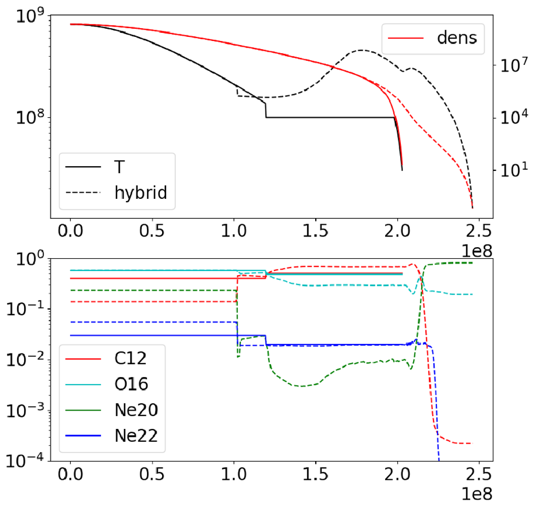
\includegraphics[width=\columnwidth]{figures/initial_conds.png}
\caption{\label{fig:init_conds}
Temperature, density, and  composition profiles of the one-dimensional hybrid 
progenitor WD. The central temperature and density were the same as
the traditional C/O progenitor model. 
The peak temperature of the hybrid model is at the center of the star, 
so both the hybrid and traditional models could share the same 
	central ignition initial conditions.
}
\end{figure}
In both models, and unlike the hybrid models of~\citet{willcoxetal2016}, the central
temperature was the highest at the center of the star and accordingly the simulations 
began with central ignitions. 


\subsection{Two-dimensional Initial Conditions From One-dimensional Models}

The initial progenitor models for the two-dimensional simulations were
created from the one-dimensional \MESA\ models by mapping the one-dimensional
models onto the two-dimensional domain while 
preserving hydrostatic equilibrium.
As described above, the flame capturing scheme with progress
variables describing the evolution as the material burns. The \MESA\
models, however, relied on a detailed reaction network that included
many species. Accordingly, the process of creating the two-dimensional
models for \FLASH\ required aggregating some of the species abundances.
As with much of this study, we applied the 
techniques of~\citet{willcoxetal2016}.


The process of mapping the \MESA\ models began by converting 
the \MESA\ model to a uniform grid of $4$~km resolution. \MESA\ 
quantities in zones with spacing less than $4$~km 
were mass-weighted averaged and a quadratic interpolation
was used to calculate quantities for the case of \MESA\ zones having
a spacing greater than $4$~km. At this point, 
abundances of nuclides from the \MESA\ models were aggregated
into the abundances tracked by the flame capturing scheme in
\FLASH.
The most abundant isotopes in the model were \C{12}, \Ox{16},
and \Ne{20}, which are symmetric (the number of neutrons 
equals the number of protons). Similarly to~\citet{willcoxetal2016}, 
other neutron-rich isotopes in the initial model were combined into 
\Ne{22}, which serves as a proxy for metallicity. The aggregation
account for the $Y_e$ of the full set of nuclides, \Ne{20} 
and \Ox{16} were constrained to be in the same ratio in both 
sets of abundances. \figref{fig:init_conds} shows the initial
profile of the one-dimensional models.

The original \MESA\ model was in equilibrium, but to ensure
the uniformly-gridded model was in hydrostatic equilibrium we 
constructed the appropriate pressure profile. This was done by
integrating for the pressure in each zone from the central point up, 
accounting for the local acceleration of gravity, temperature,
composition, and the mass below and enclosed by the zone. As
with \citet{willcoxetal2016} we used
EOS routine from 
\CASTRO\ ~\citep{timmes.swesty:accuracy,castro1}.\footnote{The 
Helmholtz EOS table used in \CASTRO\ is in the public BoxLib 
Microphysics repository at
  \url{https://github.com/BoxLib-Codes/Microphysics.git} (commit 
  hash $\mathrm{45ed859b6c1dc80d831d93f9728986d6ad6e1ddc}$).} As 
 with the models in \citet{willcoxetal2016},this procedure produced 
 a structure that was stable in \FLASH, with fluctuations in central
density less than $3\%$, for at least $5$ seconds with no energy
deposition.

\subsection{DDT Process and Suits of Explosions}

The simulations performed for this study consisted to a suite of
{\color{red} 35 CHECK THIS! 40?} two-dimensional simulations of 
thermonuclear supernova
explosions from hybrid C-O-Ne progenitors in the DDT explosion paradigm. These 
were compared to a suite of supernova simulations from traditional
C-O progenitors. In both suites, the simulation
begins with a progenitor model mapped to the two-dimensional 
\FLASH\ grid. The burning is initiated with a ``match head,'' a region 
in the white dwarf's center that is fully burned to nuclear statistical
equilibrium (NSE). 
This initially burned region ignites a deflagration, a subsonic
flame, and because the match head was perturbed it is unstable to
the Rayleigh-Taylor instability with the result that buoyant plumes 
rise. The star is partially consumed during this deflagration phase,
and the star responds by expanding.
When a plume reaches a specified density,
a detonation is initiated, and the simulation continues until 
the expanding star reaches low densities at which point burning
effectively ends. The paragraphs in this section provide details
of the implementation of this method.


{\color{red} ARE THE BELOW NUMBERS CORRECT?}
The C-O and C-O-Ne models have the same central density
and temperature $7 \times 10^8$~K, respectively.
The C-O model had core composition of (\C{12} = 0.4, 
\Ne{20} = 0.03, \Ox{16} = 0.57) and envelope composition 
of (\C{12} = 0.5, \Ne{20} = 0.02, \Ox{16} = 0.48). 
The C-O-Ne model had core composition of (\C{12} = 0.X, 
\Ne{20} = 0.XX, \Ox{16} = 0.XX) and envelope composition 
of (\C{12} = 0.XX, \Ne{20} = 0.0X, \Ox{16} = 0.XX). 
The profiles of the two-dimensional models match those of
the one-dimensional models (shown in \figref{fig:init_conds})
up to very slight errors from the mapping process. {\color{red}
OMIT THIS LAST SENTENCE? DONT HAVE A FIGURE}

The simulations were performed in two-dimensional $\mathrm{z-r}$
cylindrical coordinates, extending radially from 0 to
$65,536$~\km\ and along the axis of symmetry from $-65,536$~\km\ to
$65,536$~\km. The maximum refinement level of the adaptive mesh 
corresponded to $4$~\km\ resolution, which previous study has shown is
is a good balance between efficiency and 
accuracy~\citep{townsley.calder.ea:flame,townetal2009}.
This resolution and geometry was used in previous studies
allowing direct comparison to previous results~\citep{kruegetal12}.

The ignition of the deflagration via a match head followed the 
initialization described in~\citet{kruegetal12}, which
followed the method of~\citet{townetal2009}.
In both the hybrid and traditional cases, the match head had a 
nominal radius of $150$~km before 
a different randomly-seeded perturbation was applied to the 
match head for each of the 35 simulations in both suites. {\color{red}
IS THIS RIGHT- BOTH USED THE SAME REALIZATIONS?}
The perturbation to the sphere's surface is a set of
spherical harmonic functions with randomly chosen amplitudes, and
each set of perturbations is referred to as a ``realization." 
These perturbations have been shown to reproduce 
the scatter in \Ni{56} 
yield from \SNeIa\ \citet{townetal2009}.


The transition from deflagration to detonation again follows
the previous studies, which assumed the transition location
is parameterized by the fuel density $\rho_{\mathrm{DDT}}$.
When a rising
plume reaches the threshold density, in this case
$\rho_{\mathrm{DDT}} = 10^{7.2}~\grampercc$, 
a $12$~\km\ a region of fuel, (\C{12} and \Ne{20}, if present) is
fully burned $32$~\km\ radially outwards from the flame. This
instantaneous burning in the region of this size provides conditions
to generate the shock and support the detonation at the chosen
threshold density.  Multiple DDT points may arise, but they are
constrained to be at least $200$~\km\ apart. The choice of DDT
in the suite has been shown to be high enough to ensure 
the robust ignition of a detonation shock.

Once the detonation starts, the remaining fuel at densities
high enough for the detonation to propagate is quickly consumed.
The simulations were run to 4.0 s, at which time burning 
has effectively ceased. 


\section{Results}

We frame the presention of the results of the suites of simulations 
principally in terms of the yield of \Ni{56}, the source of 
the light curve of an event. \Ni{56} thus serves as a proxy
for the brightness of an explosion and comparison of the yields
is equivalent to comparing the brightness events. The
yields estimated from $Y_e$ and the NSE progress
variable, by assuming the composition in NSE is \Ni{56} plus equal
parts \Fe{54} and \Ni{58}, as described in
\citet{townetal2009,Meaketal09}.

\begin{figure}
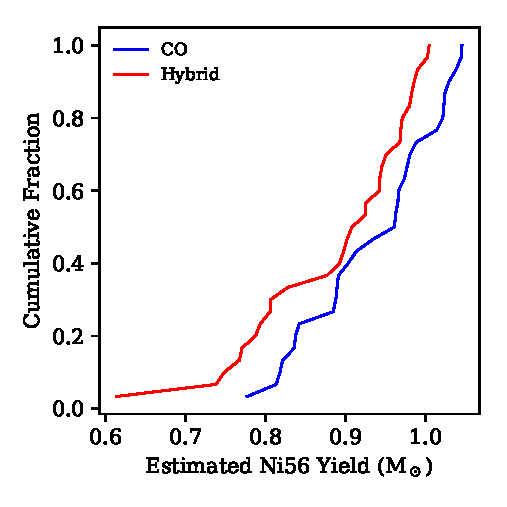
\includegraphics[width=\columnwidth]{figures/ni56_yield_cum_dist.pdf}
\caption{\label{fig:cumdist}
The cumulative distribution of the \Ni{56} yield for explosions from
C-O and hybrid C-O-Ne models. The hybrid results are shown in red, and the CO
results are shown in blue. The curve for the hybrid models is shifted 
to the left, indicating that explosions from hybrid progenitors produce
less \Ni{56} than explosions from traditional C-O models. 
}
\end{figure}
The cumulative distribution of the \Ni{56} yield for explosions from
C-O and hybrid C-O-Ne models is presented in \ref{fig:cumdist}. 
The figure shows that the hybrid models consistenly have a higher
cumulative fraction at a given mass of \Ni{56}, which indicates
that the yields of \Ni{56} are consistenly lower in explosions 
from hybrid progenitors. {\color{red} CHECK/EXPAND THIS}

\begin{figure}
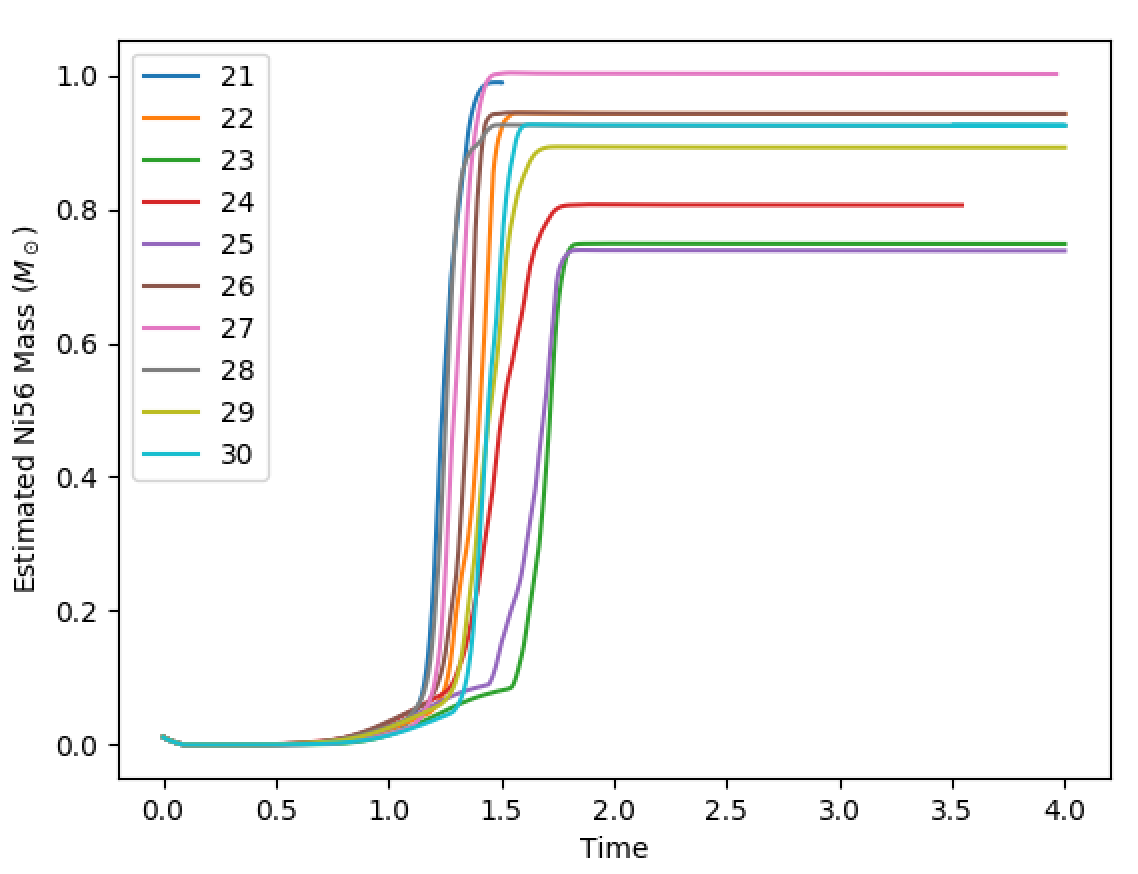
\includegraphics[width=\columnwidth]{figures/ni56_vs_time_hybrid.png}
\caption{\label{fig:nithybrid}
Estimated \Ni{56} mass vs.\ time for ten hybrid model explosion simulations. 
Shown are realizations 21-30. 
}
\end{figure}
\begin{figure}
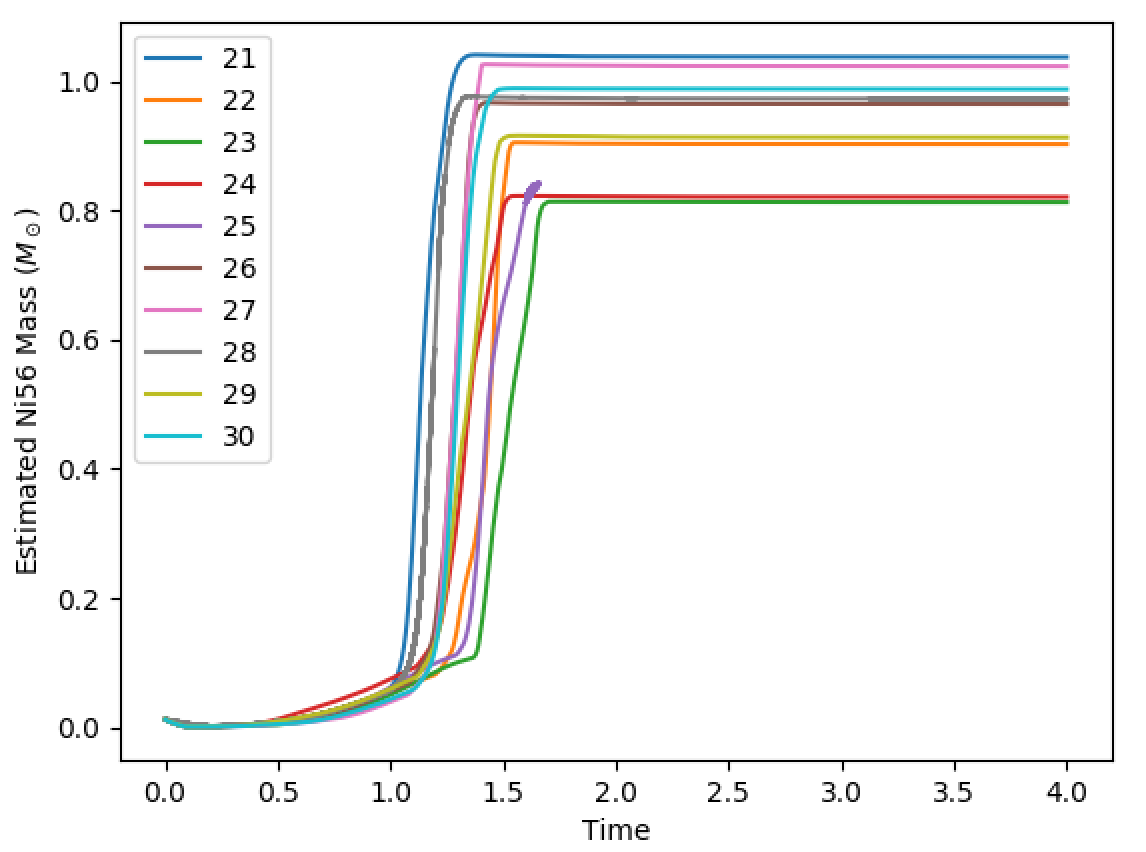
\includegraphics[width=\columnwidth]{figures/ni56_vs_time_CO.png}
\caption{\label{fig:nitco}
Estimated \Ni{56} mass vs.\ time for ten C-O model explosion simulations.
Shown are realizations 21-30. 
}
\end{figure}

The estimated production of \Ni{56} as a function of simulation time
for 10 simulations of explosions from the hybrid progenitor is shown
in Figure \ref{fig:nithybrid} and from the traditional C-O progenitor is
shown in Figure \ref{fig:nitco}.
The figures show that the final estimated \Ni{56} for the C-O model is
slightly larger then the hybrid model. Therefore, the C-O produces more
\Ni{56}. The hybrid model has a larger range then the C-O model. Also, on
average, the CO model reaches the DDT phase sooner then the hybrid model.
Both figures show that production of \Ni{56} effectively ceases (the
curves flatten out) well before the end of the simulations at 
$4.0$~\second. Also, the figures show that a few simulations
did not complete. {\color{red} OFFER A WHY?}

The degree of expansion was found using the time at which the first
detonation point occurred, and the mass at density less then 2e7 g/cc. The
estimated \Ni{56} Yield is the final estimated mass of the model.

\begin{figure}
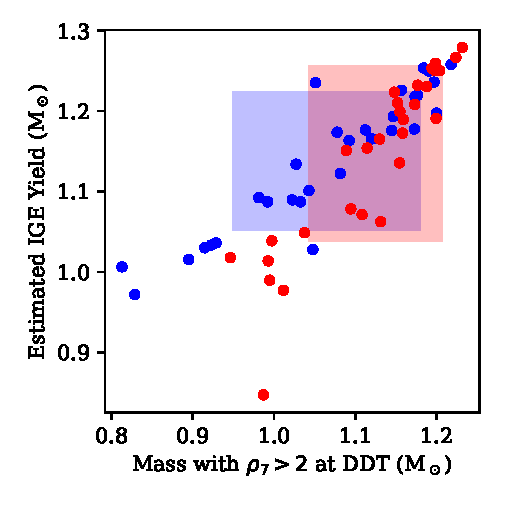
\includegraphics[width=\columnwidth]{figures/ni56_yield_vs_mass_at_high_dens.pdf}
\caption{\label{fig:masshighdens}
Final estimated IGE {\color{red} 
TO BE SURE- NOT \Ni{56} AS FIGURE IS LABELED?} yield 
vs.\ mass {\color{red} above} $2\times 10^7~\grampercc$
at the time of the first DDT in a simulation.  Individual 
realizations are shown (C-O-NE
progenitors in red, C-O in blue) along with rectangles of length
$\pm 1 \sigma$ along each axis and centered at their average values 
for C-O and C-O-Ne.
}
\end{figure}

Figure \ref{fig:masshighdens} compares the final yield of IGE elemets
for the C-O and C-O-Ne simulation suites with the amount of expansion of the
WD during the deflagration phase. The amount of expansion is 
characterized by the mass above $2 \times 10^7~\grampercc$ at the 
time of the DDT, with more high-density mass
indicating less expansion during deflagration. The averages of both
the C-O and C-O-Ne suites along both axes are indicated by the shaded
regions with $\pm1\sigma$ widths. 

As expected from previous studies, the trend for both C-O and C-O-Ne
models is that less expansion during the deflagration phase results in
greater IGE yields, because less expansion gives more high
density fuel to be consumed in the detonation.
being more high density fuel for the detonation to consume. 
As the amount of expansion increases (the less
mass above $2 \times 10^7 \grampercc$), 
for a similar amount of expansion, the C-O
models tend to yield greater IGE mass. Following 
\citet{willcoxetal2016}, we interpret
the lower IGE yield in C-O-Ne models as resulting 
from the lower \C{12} abundance and the fact that given
similar fuel density, the \Ne{20}-rich fuel will burn to cooler
temperatures than fuel in the C-O models. The result is
slower burning to IGE and thus a lower IGE yield.

\begin{figure}
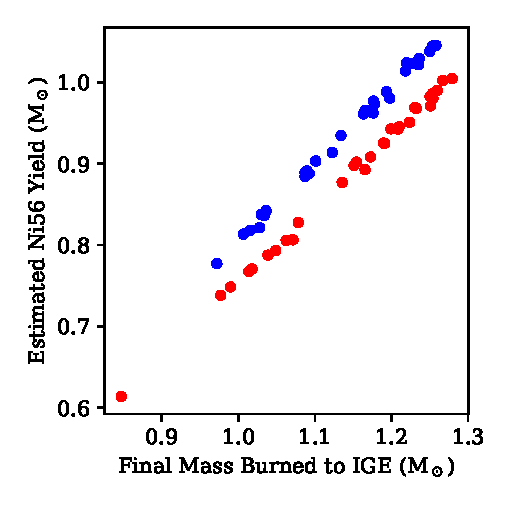
\includegraphics[width=\columnwidth]{figures/FMBTI_v_Ni56Yield_plot.pdf}
\caption{\label{fig:conversion}
	The conversion of \Ni{56} to IGEs are more pronounced in my case. There are two assumptions as to why figure 6 is more pronounced in my paper then in Dons. 
First is that higher critical density leads to higher electron capture resulting in less Ni56 produced. Figure 4 shows that CO model has a stronger electron capture then the hybrid model. The second is that the central ignition leads to early burning at higher density. Both of these cases lead to more electron capture resulting in a larger difference in evolution between the models.
NEW: Production of 56Ni and mass burned to IGEs for CO (red) and
hybrid CONe (green) WD realizations. SAME AS DON'S FIG 18
}
\end{figure}
Figure \ref{fig:conversion} shows the estimated \Ni{56} yields 
across the range of masses burned to IGE
for all C-O and C-O-Ne realizations at the end 
of the simulaitons ($4.0$~\second),
at which point the total mass burned to \Ni{56} had become constant.


\begin{figure}
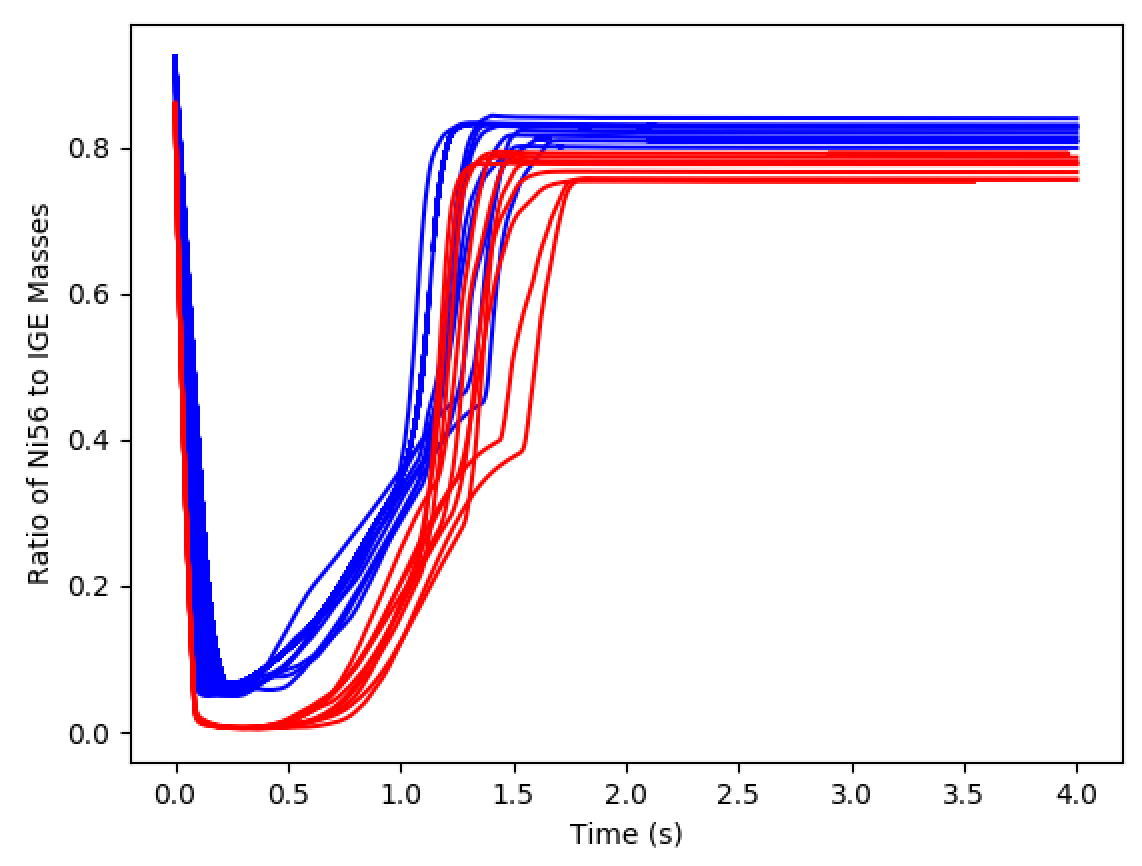
\includegraphics[width=\columnwidth]{figures/compare_ratio_v2.png}
\caption{\label{fig:compare_ratio}
Figure 8 shows the evolution of the materials for both models. It is determined that the CO model had the greatest amount of Ni56, then the other IGE materials, compared to the hybrid model.  
SAME AS DON'S FIGURE 19.
}
\end{figure}

\begin{figure}
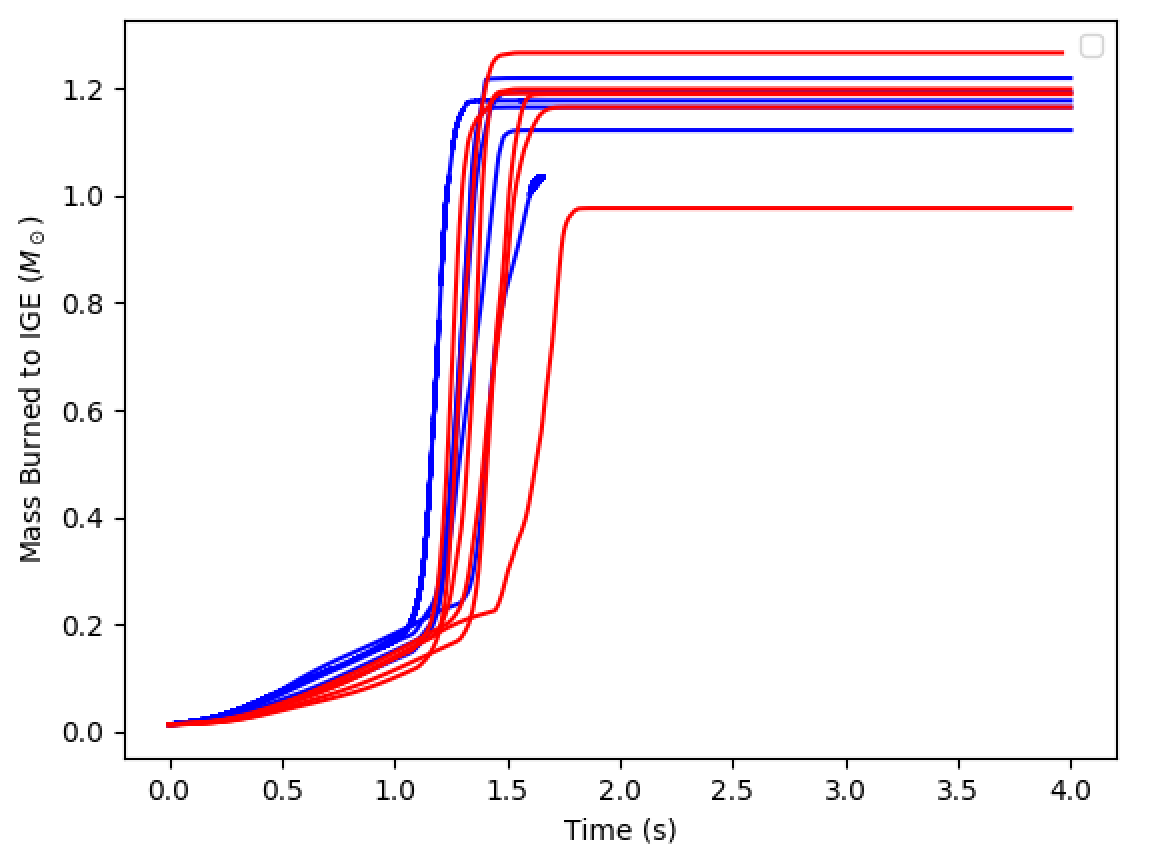
\includegraphics[width=\columnwidth]{figures/compare_burned_mass_v2.png}
\caption{\label{fig:compare_burned}
SAME AS DON'S FIGURE 20.
C/O blue hybrid red.
Note that one of the C/O simulations presented did not complete.
}
\end{figure}

\section{Discussion and Conclusion}


The conversion of \Ni{56} to Iron group elements are more pronounced in my
case. There are two assumptions as to why figure 6 is more pronounced
in my paper then in Dons.  First is that higher critical density leads
to higher electron capture resulting in less \Ni{56} produced. The second
is that the central ignition leads to early burning at higher density.


As the star burns mass, the surface area grows, resulting in a decrease
in density. The results show that the models that burned less mass during
the deflagration phase, expand less, produce more \Ni{56}. This is because
the density rich mass the model has at the DDT point is the ‘fuel’
it needs to produce \Ni{56}. Therefore, the more mass, the more Ni-56. On
average, the CO model, shown in figure 4, reaches the DDT faster then
the hybrid model. Figures 3 and 4 show that the hybrid model has a wider
range of estimated \Ni{56} mass suggesting a greater range of burned mass
and expansion during the deflagration phase.

This work was supported in part by the U.S.\ Department of Energy under
grant DE-FG02-87ER40317 and in part by the U.S.\ National Science Foundation
via a supplement to grant AST-1211563. 
Support also came from the Data + Computing = Discovery summer program at
the Institute for Advanced Computational Science at Stony Brook University.
The software used in this work was developed in part by the DOE-supported 
ASC/Alliances Center for Astrophysical Thermonuclear Flashes at the 
University of Chicago. 
The source code used for
these studies is available as a package compatible with the
current Flash code from \url{http://astronomy.ua.edu/townsley/code.}
Results in this
paper were obtained using the high-performance computing system at the
Institute for Advanced Computational Science at Stony Brook
University. 


%%%%%%%%%%%%%%%%%%%%%%%%%%%%%%%%%%%%%%%%%%%%%%%%%%%%%%%%%%%%%%%%%%
% SOFTWARE
%% \software{
%%   FLASH \citep{Fryxetal00},
%%   CASTRO \citep{castro1},
%%   MESA \citep{mesa1},
%%   Matplotlib \citep{http://dx.doi.org/10.5281/zenodo.44579}
%% }

%%%%%%%%%%%%%%%%%%%%%%%%%%%%%%%%%%%%%%%%%%%%%%%%%%%%%%%%%%%%%%%%%%
\bibliography{master}


\end{document}

